\documentclass[crop,tikz]{standalone}
\usepackage{amsfonts}
\usetikzlibrary{shapes}
\usetikzlibrary{arrows}
\usetikzlibrary{positioning}
\begin{document}
 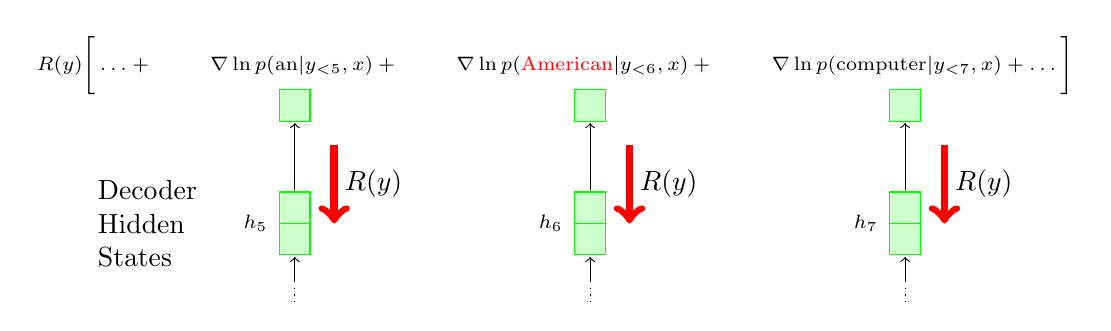
\begin{tikzpicture}[
    record/.style={rectangle,draw=black,anchor=north west,text width=42mm,
                   font=\scriptsize},
    beam/.style={rectangle,draw=black,anchor=north west,text width=36mm,
                 font=\scriptsize},
    table/.style={anchor=north west,rotate=90,font=\tiny},
    dot/.style={circle,draw=black,fill=white,inner sep=.75pt},
  hid/.style 2 args={
    rectangle split,
    draw=#2,
    rectangle split parts=#1,
    fill=#2!20,
    outer sep=.25mm},
  mlp/.style 2 args={
    rectangle split,
    rectangle split horizontal,
    draw=#2,
    rectangle split parts=#1,
    fill=#2!20,
b
    outer sep=.25mm}
 ]

%\node[anchor=west] at (2,5) {Speaker: $y \sim p(\cdot|x)\quad\quad\quad\quad$ Listener: $ \hat{x} \sim q(\cdot|y)$};
%\node[anchor=west] at (2,4.5) {Reward: $R(y) = q(x|y)\quad\quad$~ Objective: $  \mathcal{L} = \mathbb{E}_{y\sim p(\cdot|x) }\left[ R(y) \right]  $};
%
%\node[anchor=west] at (2,3.75) {Approx. Gradient: $\nabla\mathcal{L} \approx \frac{1}{n} \sum_{i=1}^n R(y^{(i)}) \nabla \ln p(y^{(i)}|x)$};

\node[text width=2cm] at (1.75, 1) {Decoder Hidden States};
%\draw[black] (0,0) rectangle (11,6);
\node[anchor=west] at (-0.15,3) {\scriptsize $R(y) \Big[ \ldots 
+ {\color{white} R(y_5)} \nabla\ln p(\textrm{an}|y_{<5},x)
+ {\color{white} R(y_6)} \nabla\ln p(\textrm{\color{red}American}|y_{<6},x)
+ {\color{white} R(y_7)} \nabla\ln p(\textrm{computer}|y_{<7},x) + \ldots \Big]$};


 \node[hid={2}{green}] (h1) at (3.25, 1) {};
 \node (s) at (2.75, 1) {\scriptsize $h_5$};
  \draw[->,red,line width=1mm] (3.75, 2) to (3.75, 1);
\node at (4.25, 1.5) {$R(y)$};
  \draw[-,black,dotted] (3.25, 0) to (3.25, .25);
  \draw[->,black] (3.25, .25) to (h1.south);
 \node[hid={1}{green}] (p1) at (3.25, 2.5) {};
\draw[->,black] (h1.north) to (p1.south);



 \node[hid={2}{green}] (h2) at (7, 1) {};
 \node (s) at (6.5, 1) {\scriptsize $h_6$};
  \draw[->,red, line width=1mm] (7.5, 2) to (7.5, 1);
\node at (8, 1.5) {$R(y)$};
  \draw[-,black,dotted] (7, 0) to (7, .25);
  \draw[->,black] (7, .25) to (h2.south);
 \node[hid={1}{green}] (p2) at (7, 2.5) {};
\draw[->,black] (h2.north) to (p2.south);

 \node[hid={2}{green}] (h3) at (11, 1) {};
 \node (lbl3) at (10.5, 1) {\scriptsize $h_7$};
  \draw[->,red,line width=1mm] (11.5, 2) to (11.5, 1);
\node at (12, 1.5) {$R(y)$};
  \draw[-,black,dotted] (11, 0) to (11, .25);
  \draw[->,black] (11, .25) to (h3.south);
 \node[hid={1}{green}] (p3) at (11, 2.5) {};
\draw[->,black] (h3.north) to (p3.south);


%\node at (5.45,5) {\scriptsize $R(y) \Big[~~~~~~~~~~~~~~~~~~~~~~~~~~~~~~~~~~~~~~~~~~~~~~~~~~~~~~~~~~~~~~~~~~~~~~~~~~~~~~~~~~~~~~~~~~~~~~~~~~~~~~~~~~~~~ \Big]$};
%\node[circle,black] at (2,5) {\scriptsize $\ldots + \nabla \ln p(\textrm{an}|y_{<5},x)$ };
%\node[circle,black] at (3.4,5) {\scriptsize $+$ };
%\node[circle,black] at (5.25,5) {\scriptsize $\nabla \ln p(\textrm{American}|y_{<6},x)$ };
%\node[circle,black] at (9,5) {\scriptsize $\nabla \ln p(\textrm{computer}|y_{<7},x) + \ldots$ };
%

%    \node at (1,1) {Karen};
%?%    \node at (2.25,1) {Sp\"arck};
%?%    \node at (3.5,1) {Jones};
%?%    \node at (4.5,1) {was};
%?%    \node at (5.3,1) {an};
%?%    \node at (6.6,1) {American};
%?%    \node at (8.5,1) {computer};
%?%    \node at (10.3,1) {scientist.};
%?
%? \node[anchor=west] at (-3.69, .5) {$y = $~~~~~~~ Karen ~~~~ Sparck ~~~~ Jones ~~~~~~ was ~~~~~~~~~ an ~~~ American~ computer~~ scientist};
%?    \node at (1, 0) {$ \nabla \mathbb{E}_{p(\cdot|x)}\left[R(y)\right] 
%?    \approx R(y) \nabla \log p(y|x) =  R(y) \left[  \nabla \log p_1 
%?        + \nabla \log p_2 + \nabla \log p_3 
%?        + \nabla \log p_4 + \nabla \log p_5 
%?        + \nabla \log p_6 + \nabla \log p_7
%?        + \nabla \log p_8 \right] $};
%? \node[anchor=west] at (-3.69, -.5) {$R(y_1) \nabla \log p_1 +
%? R(y_2) \nabla \log p_2 +
%?R(y_3) \nabla \log p_3 +
%?R(y_4) \nabla \log p_4 +
%?R(y_5) \nabla \log p_5 +
%?R(y_6) \nabla \log p_6 +
%?R(y_7) \nabla \log p_7 +
%?R(y_8) \nabla \log p_8  $};
%?
%?
%?%    \node at (1, 0) {$ \nabla \mathbb{E}_{p(\cdot|x)}\left[R(y)\right] 
%?%    \approx R(y) \nabla \log p(y|x) =  R(y) \left[  \nabla \log p(Karen|x) 
%?%        + \nabla \log p(Sparck|y_{<2},x) + \nabla \log p(Jones|y_{<3},x) 
%?%        + \nabla \log p(was|y_{<4},x) + \nabla \log p(an|y_{<5},x) 
%?%        + \nabla \log p(American|y_{<6},x) + \nabla \log p(computer|y_{<7},x)
%?%        + \nabla \log p(scientist|y_{<8},x) \right] $};
%?
%?
%?  %\draw[color=black] (0,7.25) rectangle (15,0);
%?
%?%  \node[record] (r1) at (.05,4.41-.6*0) {\textbf{Name:} Karen Sp\"arck Jones};
%?  %\node[record] (r2) at (.05,4.41-.6*1) {\textbf{Born:} 26 August 1935};
%?  \node[record] (r2) at (.05,4.41-.6*1) {\textbf{Name:} Karen Sp\"arck Jones};
%?  %\node[record] (r3) at (.05,4.41-.6*2) {\textbf{Died:} 4 April 2007};
%?  \node[record] (r3) at (.05,4.41-.6*2) {\textbf{Occupation:} Computer Scientist};
%?  \node[record] (r4) at (.05,4.41-.6*3) 
%?  {\textbf{Nationality:} British};
%?       % {\textbf{Occupation:} Computer Scientist};
%? % \node[record] (r5) at (.05,4.41-.6*4) {\textbf{Nationality:} British};
%?  
%?  \node at (2.25,4.75-.6) {Table Data};
%?  \node[rectangle,densely dotted,draw=black] (gen) at (5.4, 5) {Speaker};
%?  \node[rectangle,densely dotted,draw=black] (rec) at (11.3, 5) {Listener};
%?  \node[text width=26mm,align=center] at (13.5,6.75) 
%?    {Recovered Table Data};
%?
%? \node[beam] (b2) at (6.5,3.35) 
%?    {Karen Sp\"arck Jones was a British computer scientist.};
%?
%?
%? %   \draw[-] (r1.east) to [out=0,in=180] (5,2.975);
%?    \draw[-] (r2.east) to [out=-15,in=180] (5,2.975);
%?    \draw[->] (r3.east) to (4.5,2.975) to (5.5,2.975) to  (b2.west); 
%?    \draw[-] (r4.east) to [out=15,in=180] (5,2.975);
%?  %  \draw[-] (r5.east) to [out=0,in=180] (5,2.975);
%?%    \draw[->] (5.5,2.975) to [out=0,in=180] (b1.west);
%? %   \draw[->] (5.5,2.975) to [out=0,in=180] (b3.west);
%?
%?
%?
%? \node[table] (d1) at (12.5, 3.25) 
%?    {\begin{tabular}{l} 
%?        Accountant \\ 
%?        Body Builder \\ 
%?        Comp. Scientist\\ 
%?        D \\
%?        \quad~~~~~$\vdots$ \\
%?        X-ray Tech. \\ 
%?        Y \\ 
%?        Zoologist 
%?    \end{tabular}}; 
%?
%? \node[table] (d2) at (12.5, 1-.5) 
%?    {\begin{tabular}{l} 
%?        American \\ 
%?        British\\ 
%?        Canadian \\
%?        Dutch \\
%?        \quad~$\vdots$ \\
%?        German \\ 
%?        Italian\\
%?        French \\ 
%?    \end{tabular}}; 
%?
%?%? \node[table] (d3) at (12.5, 0) 
%?%?    {\begin{tabular}{l} 
%?%?        French \\ 
%?%?        German \\ 
%?%?        British\\ 
%?%?        Italian \\
%?%?        \quad~$\vdots$ \\
%?%?        Mexican \\ 
%?%?        American \\ 
%?%?        Canadian 
%?%?    \end{tabular}}; 
%?
%?   \draw[-] (12.5,5.35) to (14.75, 5.35);
%?   \foreach \x/\ystop in {12.75/5.5,12.95/5.5,13.14/5.95,13.35/5.5,14.15/5.5,
%?                          14.35/5.5,14.55/5.5} {
%?     \draw[-] (\x,5.35) to (\x, \ystop);
%?     \node[dot] at (\x,\ystop) {};
%?   }
%?   \node at (13.8,5.5) {$\cdots$};
%?
%?
%?
%?   \draw[-] (12.5,2.5-.5) to (14.75, 2.5-.5);
%?   \foreach \x/\ystop in {12.75/2.65,12.95/3.1,13.14/2.65,13.35/2.65,14.15/2.65,
%?                          14.35/2.65,14.55/2.65} {
%?     \draw[-] (\x,2.5 - .5) to (\x, \ystop -.5);
%?     \node[dot] at (\x,\ystop - .5) {};
%?   }
%?   \node at (13.8,2.65-.5) {$\cdots$};
%?   \node at (13.75,1-.5) {\scriptsize Nationality};
%?   \node at (13.75,3.25) {\scriptsize Occupation};
%?
%?
%?   
%?%   \draw[-] (12.5,1.35) to (14.75, 1.35);
%?%   \foreach \x/\ystop in {12.75/1.5,12.95/1.5,13.14/1.5,13.35/1.5,14.15/1.5,
%?%                          14.35/1.95,14.55/1.5} {
%?%     \draw[-] (\x,1.35) to (\x, \ystop);
%?%     \node[dot] at (\x,\ystop) {};
%?%   }
%?%   \node at (13.8,1.5) {$\cdots$};
%?%
%?%    \draw[->] (b1.east) to (12.25,4.975);
%?   \draw[->] (b2.east) to (11.25,2.975) to [out=0,in=180] (d2.north);
%?   \draw[->] (11.25,2.975) to [out=0,in=180] (d1.north);
%?%    \draw[->] (b3.east) to (12.25,0.975);
%?
%?    %\draw[draw=green] (12.4,6.15) rectangle (14.85,3.25);
%?    %\draw[draw=yellow] (12.4,3.25) rectangle (14.85,1.25);
%?%    \draw[draw=red] (12.4,2.15) rectangle (14.85,0.25);
%?%    \draw[-,densely dotted] (rec.south) to [out=270,in=180] (12.25,4.975);
%?%    \draw[-,densely dotted] (rec.south) to [out=270,in=180] (12.25,2.975);
%?%    \draw[-,densely dotted] (rec.south) to [out=270,in=180] (12.25,0.975);
%?%    \draw[-,densely dotted] (gen.south) to [out=270,in=180] (b1.west);
%?%    \draw[-,densely dotted] (gen.south) to [out=270,in=180] (b2.west);
%?%    \draw[-,densely dotted] (gen.south) to [out=270,in=180] (b3.west);
%?   
%?
%Karen Sp\:arck Jones FBA (26 August 1935 – 4 April 2007) was a British computer scientist who was responsible for the concept of inverse document frequency, a technology that underlies most modern search engines.[3][4]
 \end{tikzpicture}
\end{document}
